\documentclass[a4paper,11pt]{article}

\usepackage{optscribe}

\begin{document}

\makeheader{4}                              					% lecture number
           {August 18, 2016}      			              % lecture date
           {Pratik Mishra}                     	          % Your name
           {Duality}  						% lecture title

\section{ Introduction}
In Mathematical Optimization theory, duality or the duality principle is the principle that optimization problems may be viewed from either of two perspectives, the primal problem or the dual problem. The solution to the dual problem provides a lower bound to the solution of the primal (minimization) problem \cite{Boyd2004}. This document briefly introduces Four major dual problems namely the Lagrangian dual problem, the Wolfe dual problem, the Fenchel dual problem and the Pontryagin dual problem but focusses its attention on the frequently used Fenchel dual and Lagrangian dual. 

\section{The standard Optimization problem}
\begin{definition}
The standard Optimization problem can be stated as the primal problem in the following way :

\centerline{$\underset{x \in D}{min}$  $ F_0(x)$}
\centerline{such that  $F_i(x) \leq 0$ \,\,\,\,  i=1,...,m.}
where $D$ is the Domain of the function $F_0$.\newline
\end{definition}

\begin{example}
Linear Programming (LP)\newline 
\centerline{\( \underset{\textbf{x} \in \mathbb{R}^d}{min}\) \(\textbf{a}^T\textbf{x}\) }
\newline
\newline
\centerline {such that ${\textbf{b}_\textbf{i}}^T\textbf{x} \leq \textbf{c}_\textbf{i}, \,\,\, i=1,...,n.$}
\end{example}


\section{The Dual Problem}
Following are Four dual problems in Mathematical Optimization :
\subsection{Fenchel dual problem}
In mathematics and mathematical optimization, the convex conjugate of a function is a generalization of the Legendre transformation. It is also known as Legendre-Fenchel transformation or Fenchel transformation (after Adrien-Marie Legendre and Werner Fenchel). It is used to transform an optimization problem into its corresponding dual problem, which can often be simpler to solve.

\begin{definition}
Let $X$ be a real vector space and $X^*$ be the dual space of $X$.
\end{definition} 

\begin{definition}
\(Let \,\, f : X \mapsto \mathbb{R}\,\,\,\, (X=\mathbb{R}^d)\)
\newline
 \( f^* : X^* \mapsto \mathbb{R}\) is called the fenchel dual of $f$ where \newline
 \( f^*(\vx^*) :=  sup\{ \langle \vx^*,\vx\rangle - f(\vx) | \vx \in X \} \)
\end{definition}
This definition can be interpreted as an encoding of the convex hull of the function's epigraph in terms of its supporting hyperplanes.\cite{frank}

\begin{figure}[ht!]
\centering
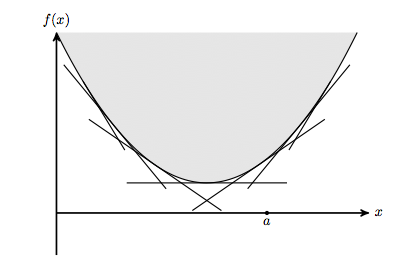
\includegraphics[width=90mm]{fd_2.png}
\caption{Deciphering function from tangent lines \newline Courtesy: http://math.stackexchange.com/questions/223235/please-explain-the-intuition-behind-the-dual-problem-in-optimization }
\end{figure}

\begin{figure}[ht!]
\centering
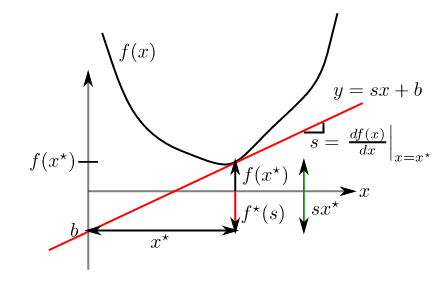
\includegraphics[width=90mm]{fd_1.png}
\caption{Graphical interpretation of Fenchel Dual  \newline Courtesy: http://www.onmyphd.com/?p=legendre.fenchel.transform }
\end{figure}


\begin{example}
The fenchel dual of an affine function \newline
\( f(\vx) = \langle \va,\vx \rangle -b, \,\, \va \in \mathbb{R}^n, b \in \mathbb{R} \) \newline
is \newline
\( f^*(\vx^*) =
 \begin{cases}
    b, & \text{if } \vx= \va\\
    \infty,              & \text{otherwise}
\end{cases}
\)
\end{example}


As Definition 4.3 and Figure 2 try to illustrate, if \(f^* (\vx^*) = -\infty\) or \( \infty \), then $\vx^*$ is not a valid slope of a tangent to $f$.

\begin{proposition}
Fenchel's Inequality \newline
For any function $f$ and its fenchel dual $f^*$,  Fenchel's inequality (also known as the Fenchel-Young inequality) holds for every $\vx \in X$ and $\vp \in X^*$ : \newline \newline
\( \langle \vp,\vx \rangle \leq f(\vx) + f^*(\vp)\) 
\cite{wiki:001}
\end{proposition}

\begin{definition}
Let \( f,f^*, X\) and  \(X^*\) as in Definition 4.3. Then, \newline
\( f^{**} (\vx) := sup\{ \langle \vx,\vx^* \rangle - f^*(\vx^*) | \vx^* \in X^* \} \) is called the double dual or biconjugate of $f$.
\cite{wiki:001}
\end{definition}

\begin{claim}
\(f=f^{**}\) if and only if $f$ is convex and lower semi-continuous.
\end{claim}

\begin{proof}
By Fenchel-Moreau Theorem.
\end{proof}

\begin{example}
Consider the function $f(x) = max(1-x,0)$. \newline
Then  \(f^*(x^*)=\begin{cases}
    x^*, & \text{if } x^* \in  [-1,0] \\
    \infty,              & \text{otherwise}
\end{cases}
\)
\newline \newline \newline
Thus \( f^{**}(x)=\underset{x^* \in [-1,0]}{sup} x^*(x-1) =f(x)\)
\end{example}

\begin{figure}[!htb]
\centering
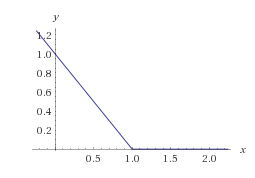
\includegraphics[width= 80mm]{fd_5.png}
\caption{Plot for the function f(x) in example 4.3\newline Courtesy : http://www.wolframalpha.com/input/?i=f(x)\%3Dmax(1-x,0)}
\end{figure}


\begin{example}
Let \( f(x) = \parallel x \parallel \) \newline \newline 
Then , \( f^*(x^*)=\begin{cases}
    1, & \text{if } \parallel x\parallel_* \leq  1 \\
    \infty,              & \text{otherwise}
\end{cases}
\)
\end{example}

\begin{remark}
The fenchel dual is also called Convex Conjugate of $f$ because, $\forall f,\,\,\,f^*$ is always convex. 
\end{remark}

\begin{remark}
Fenchel dual on a non convex function gives a smoothened version of the function that is convex.
\end{remark}

\begin{figure}[ht!]
\centering
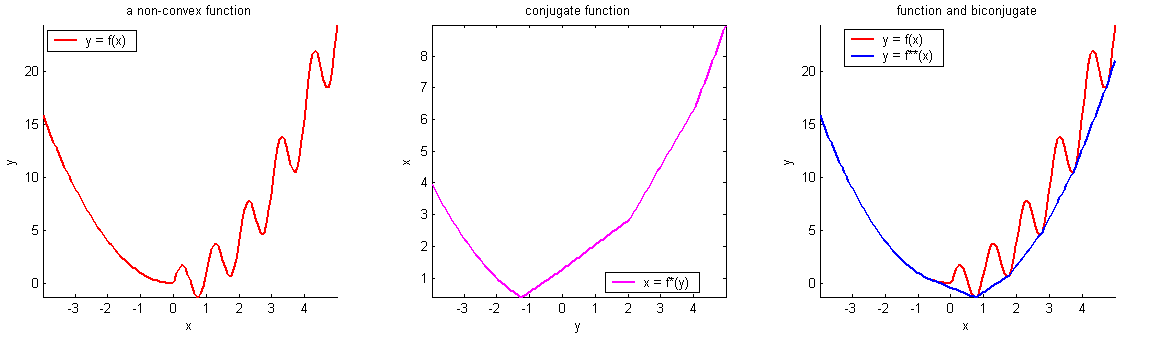
\includegraphics[width=130mm]{fd_3.png}
\caption{Illustration for Remark 4.2  \newline Courtesy :  https://msampler.wordpress.com/2009/07/08/convex-analysis/}
\end{figure}

\subsubsection{Subgradients}
In mathematics, the  subgradient  generalizes the derivative to functions which are not differentiable. 

\begin{definition}
Let $f$ be a convex function. Then, a linear function $g$ is a subgradient of $f$ at $\vx$  if , $\forall \vy$, \newline
\(f(\vy) \geq f(\vx) + \langle g,\vy-\vx \rangle \)
\end{definition}

\begin{definition}
The set of all subgradients of a function $f$ is called its subdifferential $\partial_x(f)$. 
\( \partial_x(f) = \{ g | g \text{ is a subgradient of } f \text{ at } x \}. \)  
\end{definition}

\begin{remark}
If $f$ is a differentiable function then  $\partial_x(f)$ has only 1 member, i.e, the differential.
\end{remark}

\begin{figure}[ht!]
\centering
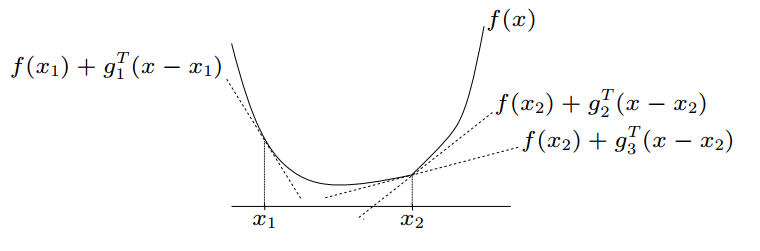
\includegraphics[width=160mm]{fd_4.png}
\caption{Subgradients of a function  \newline Courtesy : https://optimization.mccormick.northwestern.edu/index.php/Subgradient\_optimization}
\end{figure}


\begin{remark}
For non differentiable functions, the fenchel dual is defined on all directions which are subgradients of $f$ at some point.
\end{remark}

\subsection{Lagrangian dual problem}
The Lagrangian dual problem is obtained by forming the Lagrangian, using nonnegative Lagrange multipliers to add the constraints to the objective function, and then solving for some primal variable values that minimize the Lagrangian. This solution gives the primal variables as functions of the Lagrange multipliers, which are called dual variables, so that the new problem is to maximize the objective function with respect to the dual variables.\cite{wiki:002} It is a method to convert problems into unconstrained problems.
\newline
The Primal problem has already been defined in Definition 4.1
\newline

\begin{definition}
Let \(  P := \{ \vx \in X | F_i(\vx) \leq \vzero \} \) where $F_i(\vx)$ is as defined in Definition 4.1 
\end{definition}

\begin{definition}
Let \( \vp^* = \underset{\vx \in P}{min}\,\, F_0(\vx)\) where $F_0(\vx)$ is as defined in Definition 4.1
\end{definition}

\begin{definition}
The lagrangian dual function is defined in the following way : \newline \newline
\( L(X,\{\lambda_i\})= inf\{ F_0(\vx) + \sum_{i=1}^{m} \lambda_i F_i(\vx) \}\)
\end{definition}

\begin{definition}
The lagrangian dual problem can be formalized in the following way: \newline \newline
\centerline{\( \vd^*= \underset{\lambda_i \geq 0}{max} \,\,\,\,  L(X,\{\lambda_i\}) \)}
\end{definition}

\begin{theorem}
Weak Duality Theorem \newline \newline
Consider the Primal Problem P defined in Definition 4.1 and its solution $\vp^*$ defined in Definition 4.8. Also consider its Lagrangian dual problem D and its solution $\vd^*$ defined in Definition 4.10.  Then : \newline
\( \vp^* \geq \vd^* \)
\end{theorem}

\begin{proof}
 Let $\vlambda$ and $\vx$ be the feasible solutions to D and P. Then, \newline
 \( \vd^*=L(X,\vlambda)=inf\{f(\vx_1) + \vlambda^TF_i(\vx_1) | \vx_1 \in X \} \)
 \(   \leq f(\vx) + \vlambda^TF_i(\vx) \leq f(\vx) = \vp^*\)
\end{proof}

\begin{definition}
Duality Gap is defined as the difference between $\vp^*$ and $\vd^*$.
\end{definition}

\begin{theorem}
Strong Duality Theorem \newline \newline
Let $X$ be a non empty convex set in \( \mathbb{R}^n\). Let $F_0$ : $\mathbb{R}^n \mapsto \mathbb{R}$ and $F$ : $\mathbb{R}^n \mapsto \mathbb{R}^m$ be convex. Suppose there exists an $\hat{\vx} \in X$ such that $F(\hat{\vx})<\vzero$. Then \newline
\( p^* = d^* \).
\end{theorem}

\begin{proof}
For proof please refer to http://www.eng.newcastle.edu.au/eecs/cdsc/books/cce/Slides/Duality.pdf
\end{proof}

\begin{corollary}
In case of Strong Duality, Duality gap is Zero.
\end{corollary}
\begin{remark}
The above theorem is also known as Slater's condition for strong duality.
\end{remark}
\subsection{Wolfe dual problem}
In mathematical optimization, Wolfe duality, named after Philip Wolfe, is a type of dual problem in which the objective function and constraints are all differentiable functions.\newline
\begin{definition}
Wolfe dual problem \newline \newline
Consider the Lagrangian dual problem defined in Definition 4.9.\newline
Provided that the functions $F_0,F_1,F_1,...,F_m$ are continuously differentiable, the infimum occurs where the gradient is zero.
The problem \newline \newline
\( \underset{\vx,\vlambda}{maximize}\,\,\,\,F_0(\vx) + \sum_{j=1}^{m} \lambda_iF_i(\vx) \) \newline \newline
 subject to \(\nabla F_0(\vx) + \sum_{j=1}^{m} \lambda_i\nabla F_i(\vx) \) and $\vlambda \geq \vzero$ \newline \newline
is called the Wolfe dual problem.
\cite{chap3}
\end{definition}
\begin{remark}
The Wolfe dual problem is typically a non convex optimization problem.
\end{remark}

\subsection{Pontryagin duality}
In mathematics, specifically in harmonic analysis and the theory of topological groups, Pontryagin duality explains the general properties of the Fourier transform on locally compact groups, such as $\mathbb {R}$ , the circle, or finite cyclic groups. The Pontryagin duality theorem itself states that locally compact groups identify naturally with their bidual.

The subject is named after Lev Semenovich Pontryagin who laid down the foundations for the theory of locally compact abelian groups and their duality during his early mathematical works in 1934. Pontryagin's treatment relied on the group being second-countable and either compact or discrete. This was improved to cover the general locally compact abelian groups by Egbert van Kampen in 1935 and André Weil in 1940.
\cite{wiki:003}

\bibliographystyle{plainnat}
\bibliography{exampleref}

\end{document}